\documentclass{standalone}
\usepackage{tikz}
\usetikzlibrary{patterns, positioning}

\begin{document}
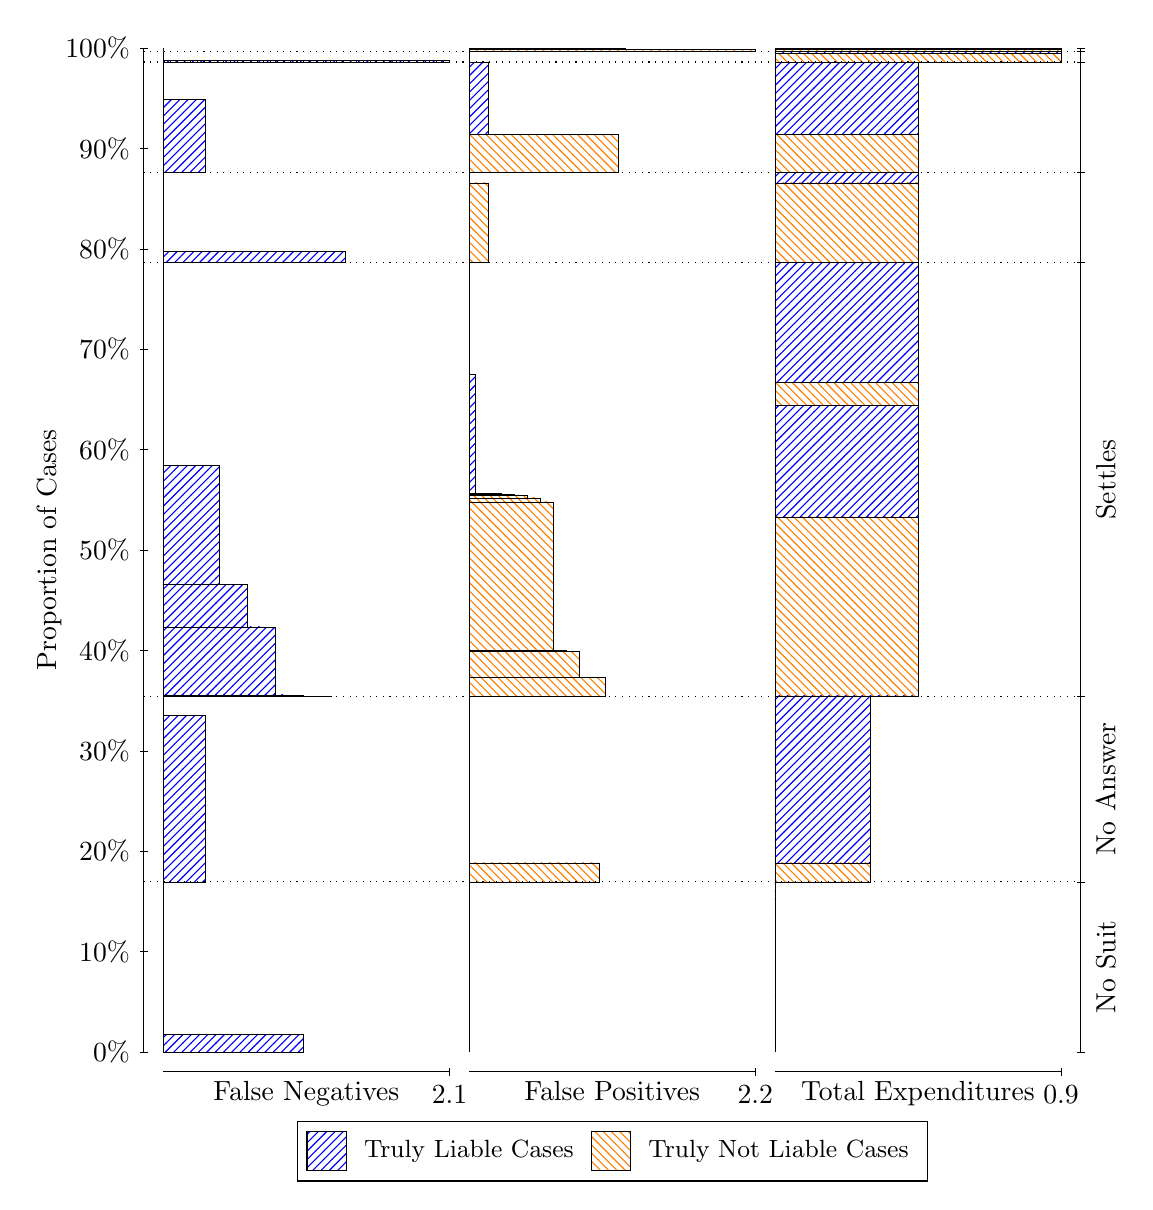
\begin{tikzpicture}
\draw[black, very thin] (1.5,1.75) -- (1.5,14.5);
\node[rotate=90, anchor=center] at (0.3, 8.125) {Proportion of Cases};
\draw[black, very thin] (1.45,1.75) -- (1.55,1.75);
\node[anchor=east] at (1.45, 1.75) {0\%};
\draw[black, very thin] (1.45,3.025) -- (1.55,3.025);
\node[anchor=east] at (1.45, 3.025) {10\%};
\draw[black, very thin] (1.45,4.3) -- (1.55,4.3);
\node[anchor=east] at (1.45, 4.3) {20\%};
\draw[black, very thin] (1.45,5.575) -- (1.55,5.575);
\node[anchor=east] at (1.45, 5.575) {30\%};
\draw[black, very thin] (1.45,6.85) -- (1.55,6.85);
\node[anchor=east] at (1.45, 6.85) {40\%};
\draw[black, very thin] (1.45,8.125) -- (1.55,8.125);
\node[anchor=east] at (1.45, 8.125) {50\%};
\draw[black, very thin] (1.45,9.4) -- (1.55,9.4);
\node[anchor=east] at (1.45, 9.4) {60\%};
\draw[black, very thin] (1.45,10.675) -- (1.55,10.675);
\node[anchor=east] at (1.45, 10.675) {70\%};
\draw[black, very thin] (1.45,11.95) -- (1.55,11.95);
\node[anchor=east] at (1.45, 11.95) {80\%};
\draw[black, very thin] (1.45,13.225) -- (1.55,13.225);
\node[anchor=east] at (1.45, 13.225) {90\%};
\draw[black, very thin] (1.45,14.5) -- (1.55,14.5);
\node[anchor=east] at (1.45, 14.5) {100\%};

\draw[black, very thin] (13.4,1.75) -- (13.4,14.5);
\draw[black, very thin] (13.35,1.75) -- (13.45,1.75);
\node[anchor=west] at (13.35, 1.75) {};
\draw[black, very thin] (13.35,3.9097) -- (13.45,3.9097);
\node[anchor=west] at (13.35, 3.9097) {};
\draw[black, very thin] (13.35,6.2663) -- (13.45,6.2663);
\node[anchor=west] at (13.35, 6.2663) {};
\draw[black, very thin] (13.35,11.778) -- (13.45,11.778);
\node[anchor=west] at (13.35, 11.778) {};
\draw[black, very thin] (13.35,12.924) -- (13.45,12.924);
\node[anchor=west] at (13.35, 12.924) {};
\draw[black, very thin] (13.35,14.322) -- (13.45,14.322);
\node[anchor=west] at (13.35, 14.322) {};
\draw[black, very thin] (13.35,14.459) -- (13.45,14.459);
\node[anchor=west] at (13.35, 14.459) {};
\draw[black, very thin] (13.35,14.5) -- (13.45,14.5);
\node[anchor=west] at (13.35, 14.5) {};

\draw[black, very thin, pattern color=blue, pattern=north east lines] (1.75,1.75) rectangle (3.5224,1.9772);
\draw[black, very thin, pattern color=orange, pattern=north west lines] (1.75,1.9772) rectangle (1.75,3.9097);
\draw[black, very thin, pattern color=blue, pattern=north east lines] (1.75,3.9097) rectangle (2.2817,6.0245);
\draw[black, very thin, pattern color=orange, pattern=north west lines] (1.75,6.0245) rectangle (1.75,6.2663);
\draw[black, very thin, pattern color=blue, pattern=north east lines] (1.75,6.2663) rectangle (3.8768,6.2676);
\draw[black, very thin, pattern color=blue, pattern=north east lines] (1.75,6.2676) rectangle (3.6996,6.2681);
\draw[black, very thin, pattern color=blue, pattern=north east lines] (1.75,6.2681) rectangle (3.5224,6.2752);
\draw[black, very thin, pattern color=blue, pattern=north east lines] (1.75,6.2752) rectangle (3.3451,6.2752);
\draw[black, very thin, pattern color=blue, pattern=north east lines] (1.75,6.2752) rectangle (3.3451,6.2859);
\draw[black, very thin, pattern color=blue, pattern=north east lines] (1.75,6.2859) rectangle (3.1679,7.1438);
\draw[black, very thin, pattern color=blue, pattern=north east lines] (1.75,7.1438) rectangle (2.9907,7.1488);
\draw[black, very thin, pattern color=blue, pattern=north east lines] (1.75,7.1488) rectangle (2.8134,7.6866);
\draw[black, very thin, pattern color=blue, pattern=north east lines] (1.75,7.6866) rectangle (2.6362,7.6889);
\draw[black, very thin, pattern color=blue, pattern=north east lines] (1.75,7.6889) rectangle (2.4589,9.2011);
\draw[black, very thin, pattern color=orange, pattern=north west lines] (1.75,9.2011) rectangle (1.75,11.778);
\draw[black, very thin, pattern color=blue, pattern=north east lines] (1.75,11.778) rectangle (4.0541,11.914);
\draw[black, very thin, pattern color=orange, pattern=north west lines] (1.75,11.914) rectangle (1.75,12.924);
\draw[black, very thin, pattern color=blue, pattern=north east lines] (1.75,12.924) rectangle (2.2817,13.844);
\draw[black, very thin, pattern color=orange, pattern=north west lines] (1.75,13.844) rectangle (1.75,14.322);
\draw[black, very thin, pattern color=blue, pattern=north east lines] (1.75,14.322) rectangle (5.3833,14.345);
\draw[black, very thin, pattern color=orange, pattern=north west lines] (1.75,14.345) rectangle (1.75,14.459);
\draw[black, very thin, pattern color=orange, pattern=north west lines] (1.75,14.459) rectangle (1.75,14.481);
\draw[black, very thin, pattern color=blue, pattern=north east lines] (1.75,14.481) rectangle (1.75,14.5);
\draw[black, very thin, pattern color=orange, pattern=north west lines] (5.6333,1.75) rectangle (5.6333,3.6825);
\draw[black, very thin, pattern color=blue, pattern=north east lines] (5.6333,3.6825) rectangle (5.6333,3.9097);
\draw[black, very thin, pattern color=orange, pattern=north west lines] (5.6333,3.9097) rectangle (7.2848,4.1515);
\draw[black, very thin, pattern color=blue, pattern=north east lines] (5.6333,4.1515) rectangle (5.6333,6.2663);
\draw[black, very thin, pattern color=orange, pattern=north west lines] (5.6333,6.2663) rectangle (7.3674,6.5086);
\draw[black, very thin, pattern color=orange, pattern=north west lines] (5.6333,6.5086) rectangle (7.2023,6.5113);
\draw[black, very thin, pattern color=orange, pattern=north west lines] (5.6333,6.5113) rectangle (7.0371,6.8366);
\draw[black, very thin, pattern color=orange, pattern=north west lines] (5.6333,6.8366) rectangle (6.872,6.8508);
\draw[black, very thin, pattern color=orange, pattern=north west lines] (5.6333,6.8508) rectangle (6.7068,8.7353);
\draw[black, very thin, pattern color=orange, pattern=north west lines] (5.6333,8.7353) rectangle (6.5417,8.786);
\draw[black, very thin, pattern color=orange, pattern=north west lines] (5.6333,8.786) rectangle (6.5417,8.7862);
\draw[black, very thin, pattern color=orange, pattern=north west lines] (5.6333,8.7862) rectangle (6.3765,8.8231);
\draw[black, very thin, pattern color=orange, pattern=north west lines] (5.6333,8.8231) rectangle (6.2114,8.8282);
\draw[black, very thin, pattern color=orange, pattern=north west lines] (5.6333,8.8282) rectangle (6.0462,8.8431);
\draw[black, very thin, pattern color=blue, pattern=north east lines] (5.6333,8.8431) rectangle (5.7159,10.355);
\draw[black, very thin, pattern color=blue, pattern=north east lines] (5.6333,10.355) rectangle (5.6333,11.778);
\draw[black, very thin, pattern color=orange, pattern=north west lines] (5.6333,11.778) rectangle (5.8811,12.787);
\draw[black, very thin, pattern color=blue, pattern=north east lines] (5.6333,12.787) rectangle (5.6333,12.924);
\draw[black, very thin, pattern color=orange, pattern=north west lines] (5.6333,12.924) rectangle (7.5326,13.402);
\draw[black, very thin, pattern color=blue, pattern=north east lines] (5.6333,13.402) rectangle (5.8811,14.322);
\draw[black, very thin, pattern color=orange, pattern=north west lines] (5.6333,14.322) rectangle (5.6333,14.436);
\draw[black, very thin, pattern color=blue, pattern=north east lines] (5.6333,14.436) rectangle (5.6333,14.459);
\draw[black, very thin, pattern color=orange, pattern=north west lines] (5.6333,14.459) rectangle (9.2667,14.481);
\draw[black, very thin, pattern color=blue, pattern=north east lines] (5.6333,14.481) rectangle (7.6152,14.5);
\draw[black, very thin, pattern color=orange, pattern=north west lines] (9.5167,1.75) rectangle (9.5167,3.6825);
\draw[black, very thin, pattern color=blue, pattern=north east lines] (9.5167,3.6825) rectangle (9.5167,3.9097);
\draw[black, very thin, pattern color=orange, pattern=north west lines] (9.5167,3.9097) rectangle (10.728,4.1515);
\draw[black, very thin, pattern color=blue, pattern=north east lines] (9.5167,4.1515) rectangle (10.728,6.2663);
\draw[black, very thin, pattern color=orange, pattern=north west lines] (9.5167,6.2663) rectangle (11.333,6.269);
\draw[black, very thin, pattern color=blue, pattern=north east lines] (9.5167,6.269) rectangle (11.333,6.2713);
\draw[black, very thin, pattern color=orange, pattern=north west lines] (9.5167,6.2713) rectangle (11.333,8.546);
\draw[black, very thin, pattern color=blue, pattern=north east lines] (9.5167,8.546) rectangle (11.333,9.9573);
\draw[black, very thin, pattern color=orange, pattern=north west lines] (9.5167,9.9573) rectangle (11.333,10.257);
\draw[black, very thin, pattern color=blue, pattern=north east lines] (9.5167,10.257) rectangle (11.333,11.778);
\draw[black, very thin, pattern color=orange, pattern=north west lines] (9.5167,11.778) rectangle (11.333,12.787);
\draw[black, very thin, pattern color=blue, pattern=north east lines] (9.5167,12.787) rectangle (11.333,12.924);
\draw[black, very thin, pattern color=orange, pattern=north west lines] (9.5167,12.924) rectangle (11.333,13.402);
\draw[black, very thin, pattern color=blue, pattern=north east lines] (9.5167,13.402) rectangle (11.333,14.322);
\draw[black, very thin, pattern color=orange, pattern=north west lines] (9.5167,14.322) rectangle (13.15,14.436);
\draw[black, very thin, pattern color=blue, pattern=north east lines] (9.5167,14.436) rectangle (13.15,14.459);
\draw[black, very thin, pattern color=orange, pattern=north west lines] (9.5167,14.459) rectangle (13.15,14.481);
\draw[black, very thin, pattern color=blue, pattern=north east lines] (9.5167,14.481) rectangle (13.15,14.5);
\draw[black, dotted] (1.5,3.9097) -- (13.4,3.9097);
\draw[black, dotted] (1.5,6.2663) -- (13.4,6.2663);
\draw[black, dotted] (1.5,11.778) -- (13.4,11.778);
\draw[black, dotted] (1.5,12.924) -- (13.4,12.924);
\draw[black, dotted] (1.5,14.322) -- (13.4,14.322);
\draw[black, dotted] (1.5,14.459) -- (13.4,14.459);
\draw[black, very thin] (1.75,1.5) -- (5.3833,1.5);
\node[anchor=north] at (3.5667, 1.5) {False Negatives};
\draw[black, very thin] (5.3833,1.45) -- (5.3833,1.55);
\node[anchor=north] at (5.3833, 1.45) {2.1};

\draw[black, very thin] (5.6333,1.5) -- (9.2667,1.5);
\node[anchor=north] at (7.45, 1.5) {False Positives};
\draw[black, very thin] (9.2667,1.45) -- (9.2667,1.55);
\node[anchor=north] at (9.2667, 1.45) {2.2};

\draw[black, very thin] (9.5167,1.5) -- (13.15,1.5);
\node[anchor=north] at (11.333, 1.5) {Total Expenditures};
\draw[black, very thin] (13.15,1.45) -- (13.15,1.55);
\node[anchor=north] at (13.15, 1.45) {0.9};

\node[black, centered, rotate=90] at (13.72, 2.8298) {No Suit};
\node[black, centered, rotate=90] at (13.72, 5.088) {No Answer};
\node[black, centered, rotate=90] at (13.72, 9.0221) {Settles};





\draw (7.449999999999999,1.5) node[draw=none] (baseCoordinate) {};
\begin{scope}[align=center]
        \matrix[scale=0.5, draw=black, below=0.5cm of baseCoordinate, nodes={draw}, column sep=0.1cm]{
            \node[rectangle, draw, minimum width=0.5cm, minimum height=0.5cm, pattern=north east lines, pattern color=blue] {}; &
            \node[draw=none, font=\small] (B) {Truly Liable Cases}; &
            \node[rectangle, draw, minimum width=0.5cm, minimum height=0.5cm, pattern=north west lines, pattern color=orange] {}; &
            \node[draw=none, font=\small] (B) {Truly Not Liable Cases}; \\
            };
\end{scope}

\end{tikzpicture}
\end{document}